\documentclass[../talk.tex]{subfiles}
\begin{document}

		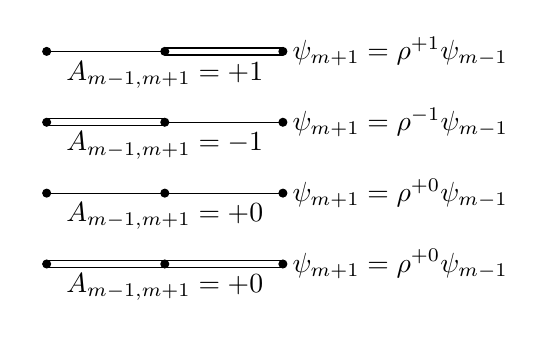
\begin{tikzpicture}[scale=1.]
    		\newcommand{\orig}{-1.5}
    		\newcommand{\trans}{1.5}
    		\newcommand{\vertspac}{.9}
    		 \newcommand{\rad}{2pt} % radii of the circles
    		
    		% set the style of the strong bonds
    		\tikzset{
    			strong/.style={
    				double,
    				double distance=\rad,
    				line width=0.5pt
    				}
    		}
    	
    		% right arrow
    		% bonds 
        	\draw[-] (\orig+\trans,0) -- (\orig+2*\trans,0) node [midway, below] {};
			\draw[strong] (\orig+2*\trans,0) -- (\orig+3*\trans,0) node [midway, below] {};	
    		% sites
		    \filldraw (\orig+1*\trans,0) circle (0.05) node [left] {} node [above] {};
		    \filldraw (\orig+2*\trans,0) circle (0.05) node [below] {$A_{m-1, m+1} = +1$};
		    \filldraw (\orig+3*\trans,0) circle (0.05) node [right] {$\psi_{m+1} = \rho^{+1} \psi_{m-1}$};
		    
		    % left arrow
		    \renewcommand{\vert}{-1*\vertspac}
		    % bonds 
        	\draw[strong] (\orig+\trans,\vert) -- (\orig+2*\trans,\vert) node [midway, below] {};
			\draw[-] (\orig+2*\trans,\vert) -- (\orig+3*\trans,\vert) node [midway, below] {};	
    		% sites
		    \filldraw (\orig+1*\trans,\vert) circle (0.05) node [left] {} node [above] {};
		    \filldraw (\orig+2*\trans,\vert) circle (0.05) node [below] {$A_{m-1, m+1} = -1$};
		    \filldraw (\orig+3*\trans,\vert) circle (0.05) node [right] {$\psi_{m+1} = \rho^{-1} \psi_{m-1}$};
		    
		    % no arrow 1
		    \renewcommand{\vert}{-2*\vertspac}
		    % bonds 
        	\draw[-] (\orig+\trans,\vert) -- (\orig+2*\trans,\vert) node [midway, below] {};
			\draw[-] (\orig+2*\trans,\vert) -- (\orig+3*\trans,\vert) node [midway, below] {};	
    		% sites
		    \filldraw (\orig+1*\trans,\vert) circle (0.05) node [left] {} node [above] {};
		    \filldraw (\orig+2*\trans,\vert) circle (0.05) node [below] {$A_{m-1, m+1} = +0$};
		    \filldraw (\orig+3*\trans,\vert) circle (0.05) node [right] {$\psi_{m+1} = \rho^{+0} \psi_{m-1}$};
		    
		    % no arrow 2
		    \renewcommand{\vert}{-3*\vertspac}
		    % bonds 
        	\draw[strong] (\orig+\trans,\vert) -- (\orig+2*\trans,\vert) node [midway, below] {};
			\draw[strong] (\orig+2*\trans,\vert) -- (\orig+3*\trans,\vert) node [midway, below] {};	
    		% sites
		    \filldraw (\orig+1*\trans,\vert) circle (0.05) node [left] {} node [above] {};
		    \filldraw (\orig+2*\trans,\vert) circle (0.05) node [below] {$A_{m-1, m+1} = +0$};
		    \filldraw (\orig+3*\trans,\vert) circle (0.05) node [right] {$\psi_{m+1} = \rho^{+0} \psi_{m-1}$};
		\end{tikzpicture}
		
\end{document}